\documentclass[10pt,a4paper]{article}
\usepackage[margin=18mm,headheight=14pt,headsep=7mm,footskip=10mm]{geometry}
\usepackage[T1]{fontenc}
\usepackage{lmodern,amsmath,booktabs,array,xcolor,fancyhdr,hyperref,pgfplots}
\pgfplotsset{compat=1.18}
\definecolor{Navy}{HTML}{17354B}\definecolor{Teal}{HTML}{166979}
\hypersetup{colorlinks=true,urlcolor=Teal,linkcolor=Teal,pdftitle={Estimated nickel tearing law},pdfauthor={MIT Rocket Team -- exploratory simulation}}
\pagestyle{fancy}\fancyhf{}
\fancyhead[L]{\small\color{Navy}MIT Rocket Team \enspace | \enspace Power board}
\fancyhead[R]{\small\color{Navy}Nickel tearing estimate}
\fancyfoot[L]{\footnotesize 5 October 2026 \enspace | \enspace Material assumptions}
\fancyfoot[R]{\footnotesize\thepage}
\renewcommand{\headrulewidth}{0.3pt}
\setlength{\parindent}{0pt}\setlength{\parskip}{5pt}\setlength{\emergencystretch}{2em}
\renewcommand{\arraystretch}{1.15}
\newcommand{\ReportHeading}[1]{\par\vspace{6pt}{\large\bfseries\color{Teal}#1}\par\vspace{3pt}}
\newcommand{\PageTitle}[1]{{\LARGE\bfseries\color{Navy}#1\par}\vspace{7pt}}
\begin{document}
\PageTitle{Estimated nickel tearing law}
{\large\color{Teal}Material-model addendum to the edge-battery lateral-pull study}\par
A usable first estimate is a \textbf{0.30 accumulated local equivalent plastic strain for damage initiation in simple tension}, followed by softening over \textbf{0.12 mm relative equivalent plastic displacement}. This is conditional on soft/annealed nickel. It is an engineering hypothesis for sensitivity analysis, not a fitted property of the user's strip and not a predicted battery breaking force.

\ReportHeading{Proposed inputs}
\begin{center}
\begin{tabular}{p{.45\linewidth}rrr}\toprule
Input & Lower value & Nominal & Upper value\\\midrule
Initiation strain at $\eta=1/3$, $\varepsilon_0$ & 0.10 & 0.30 & 0.60\\
Post-initiation displacement $u_f$ (mm) & 0.03 & 0.12 & 0.24\\
Triaxiality exponent $\beta$ & \multicolumn{3}{c}{1.5 assumed}\\
Strip thickness (mm) & \multicolumn{3}{c}{0.15 from model}\\\bottomrule
\end{tabular}
\end{center}
Vary initiation and evolution independently: the three-by-three combinations are sensitivity cases, not statistical confidence limits. The range does not bound spring-temper nickel or defects in an unknown weld.

Use the Granta annealed-sheet plasticity curve at 20$^\circ$C as the initial hardening model: 185 MPa yield and 102 exported points, ending at 530.429 MPa true stress and 0.199999 plastic strain. The source sheet is 0.787 mm thick; the modeled strip is 0.15 mm. Hardening past the exported endpoint is an additional assumption (page 3).

\ReportHeading{How the estimate was constructed}
The Granta source reports 40\% gauge-length elongation. Its logarithmic scale, $\ln(1.40)=0.336$, motivates a rounded initiation hypothesis of 0.30; it \emph{does not convert a tensile elongation measurement into a local fracture criterion}. The 0.10--0.60 interval deliberately explores that uncertainty.

Special Metals Table 13 reports 66\% and 78\% reduction in area at 21$^\circ$C for annealed Nickel 200 bars of 19 and 25.4 mm diameter [2]. Assuming locally incompressible uniaxial plastic flow gives an approximate final axial logarithmic strain
\[
\varepsilon_{\mathrm{local},f}\simeq-\ln(1-\mathrm{RA})
       =1.079\text{ to }1.514 .
\]
Using the lower bar value, an assumed localization-band width equal to the strip thickness, and the nominal onset produces
\[
u_f \simeq 0.15(1.079-0.30)=0.117\ \mathrm{mm}
          \;\longrightarrow\; \boxed{u_f=0.12\ \mathrm{mm}}.
\]
Transferring necked-bar ductility to thin sheet, ignoring neck triaxiality and using thickness as band width are substantial assumptions. This calculation supplies a scale, not a calibration. The solver's actual characteristic length must not be replaced by the strip thickness.

\clearpage
\PageTitle{Initiation and progressive damage}
Let $\eta=\sigma_m/\sigma_{\mathrm{eq}}$ be stress triaxiality, positive in hydrostatic tension. For nonnegative $\eta$, propose
\[
\varepsilon_i(\eta)=\varepsilon_0
       \exp[-1.5\max(\eta-1/3,0)],
\qquad
\omega=\int\frac{d\bar\varepsilon^p}{\varepsilon_i(\eta)}.
\]
Damage begins when $\omega=1$. The exponential is inspired by the Rice--Tracey void-growth dependence [3]; its normalization is estimated here. Holding the threshold constant below $\eta=1/3$ is a separate, uncalibrated low-triaxiality assumption. Negative-triaxiality failure is unspecified, and must not be extrapolated from this branch or interpreted as infinite fracture resistance.

\begin{center}
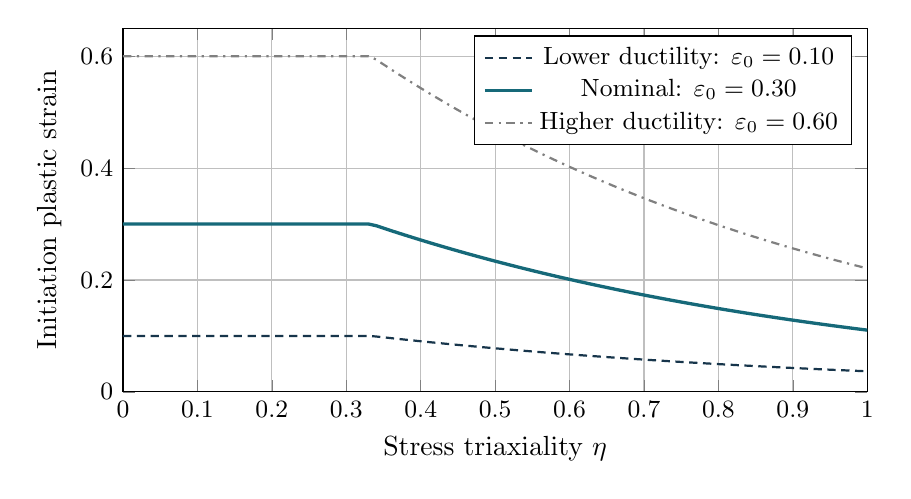
\begin{tikzpicture}
\begin{axis}[width=.91\linewidth,height=62mm,xmin=0,xmax=1,ymin=0,ymax=.65,
xlabel={Stress triaxiality $\eta$},ylabel={Initiation plastic strain},
grid=major,legend style={font=\small,at={(.98,.98)},anchor=north east},
tick label style={font=\small},samples=101]
\addplot[Navy,densely dashed,thick,domain=0:1] {.1*exp(-1.5*max(x-1/3,0))};
\addlegendentry{Lower ductility: $\varepsilon_0=0.10$}
\addplot[Teal,very thick,domain=0:1] {.3*exp(-1.5*max(x-1/3,0))};
\addlegendentry{Nominal: $\varepsilon_0=0.30$}
\addplot[gray,thick,dashdotted,domain=0:1] {.6*exp(-1.5*max(x-1/3,0))};
\addlegendentry{Higher ductility: $\varepsilon_0=0.60$}
\end{axis}
\end{tikzpicture}
\end{center}
{\small Curves are proposed assumptions drawn natively in \LaTeX; they are not test data or finite-element results.}

For constant $\eta$, the nominal threshold is 0.300 in simple tension, 0.182 at $\eta=2/3$, and 0.110 at $\eta=1$. A changing stress state requires the accumulated criterion; comparing one final strain maximum with one threshold is insufficient. The dependence omits Lode-angle effects, anisotropy and strain rate.

After initiation, use the provisional linear scalar law
\[
\bar u^p=\int_{\mathrm{onset}} L_{\mathrm{ch}}\,d\bar\varepsilon^p,\qquad
d=\min\!\left(\frac{\bar u^p}{u_f},1\right),\qquad
\boldsymbol\sigma=(1-d)\widetilde{\boldsymbol\sigma}.
\]
Here $L_{\mathrm{ch}}$ is the verified formulation's characteristic length and $\widetilde{\boldsymbol\sigma}$ is the effective elastoplastic stress. Full degradation of one material point does not establish a complete tear across a strip.

As a scale check, constant effective stress of 530 MPa with nominal linear softening gives $\tfrac12\sigma u_f\approx32$ N/mm of post-initiation work per unit area. This is an approximate consequence of the assumed law, not a measured fracture energy or the Granta toughness value.

\clearpage
\PageTitle{Reproduction and interpretation}
\ReportHeading{Hardening beyond the measured proxy}
The exported curve ends before nominal initiation in simple tension. Two explicit continuations are proposed for sensitivity:
\[
\sigma_{\mathrm{eff}}(p)=530.429\ \mathrm{MPa},
\quad\text{or}\quad
\sigma_{\mathrm{eff}}(p)=530.429
\left(\frac{p}{0.199999}\right)^{0.316193}\ \mathrm{MPa}
\quad(p>0.199999).
\]
The exponent comes from a log--log regression of the exported curve over $p\ge0.15$, with continuation anchored to its endpoint. At $p=0.30$ the power-law stress is approximately 603 MPa. Neither continuation is measured post-necking behavior; they are alternatives, not guaranteed bounds. The supplied table stops at $p=1.6$; do not silently extend it farther.

\ReportHeading{Reproducible procedure}
Run \texttt{reproduce\_estimate.py} in the companion study folder. It reads the preserved Granta CSV, computes the reduction-of-area scale and tail exponent, and writes parameter JSON, initiation and assumed-hardening CSVs, and arithmetic validation. It neither modifies nor launches ANSYS.

For a future rupture calculation, retain the two 750 N clamps, the edge-battery loading and nickel-only battery connection. Apply the candidate plasticity and damage models to the nickel, and increase prescribed battery displacement beyond the previous 0.5 mm endpoint. Track force, damage initiation, a connected tear path, and load drop separately. Compare all nine initiation/evolution pairs, both assumed hardening continuations and local mesh refinement. Include contact slip, clamp compliance and joint failure if they govern the result.

ANSYS 2026 R1 describes native ductile CDM using small-strain plasticity, tabulated initiation versus triaxiality, and characteristic-length-based evolution [4]. The large local strains proposed here require a verified compatible formulation before use. For shells its regularization length is based on in-plane integration, not thickness. No drop-in APDL implementation, native compatibility proof, material assignment or new solve has been performed for this addendum.

\ReportHeading{What the existing result establishes}
The previous refined 750 N contact case gives 8.124 N at 0.50 mm battery displacement and 0.02228 peak shell-summary plastic strain. It uses a different, illustrative bilinear material without damage. The local peak changes by 77.7\% on refinement. These results cannot be scaled into a reliable rupture force; a continued analysis with the estimated law is needed to produce a conditional numerical estimate.

\ReportHeading{Sources and provenance}
{\small
[1] Granta Selector 2026 R1, Metals plus / JAHM Curve Data, \emph{Nickel 200, annealed sheet}; exported 5 October 2026. Record source: ASM International (2002), p.~631, Fig.~Ni.001. Local audit:
\texttt{outputs/granta\_audit\_20261005/granta\_nickel\_audit.txt}.\par
[2] Special Metals, \emph{Nickel 200}, Table 13, room-temperature annealed-bar reduction in area. \href{https://www.specialmetals.com/documents/technical-bulletins/nickel-200.pdf}{Manufacturer bulletin}.\par
[3] Rice and Tracey (1969), \emph{On the ductile enlargement of voids in triaxial stress fields}, JMPS 17, 201--217. \href{https://doi.org/10.1016/0022-5096(69)90033-7}{Original theory}. The curve amplitude and low-triaxiality plateau in this addendum are analyst choices, not nickel constants from this paper.\par
[4] ANSYS 2026 R1, Material Reference, section 4.25.7, \href{https://ansyshelp.ansys.com/public/Views/Secured/corp/v261/en/ans_mat/mat_damageall.html}{Ductile Damage}.\par
Companion inputs and arithmetic:
\texttt{outputs/tearing\_estimate\_20261005/sources/}.\par
}
\end{document}

